%%%%%%%%%%%%%%%%%%%%%%%%%%%%%%%%%%%%%%%%%%%%%%%%%%%%%%%%%%%%%%%%%%%%%%%%%%%%%%%%
% TUM-Vorlage: Präsentation - Beispiele
%%%%%%%%%%%%%%%%%%%%%%%%%%%%%%%%%%%%%%%%%%%%%%%%%%%%%%%%%%%%%%%%%%%%%%%%%%%%%%%%


\begin{frame}[fragile]
\frametitle{Example of new input file}

 \begin{Verbatim}
#Random comments
# xyz-coord      velocity        mass       shape       dimensions      distance  
2
0.0 0.0 0.0      0.0 0.0 0.0     1.0
7.0 7.0 7.0      1.0 1.0 1.0     2.0e-8     CuboiD      4	5	6         3.0
# epsilon    sigma
0.1         0.2
 \end{Verbatim}

\vspace{-0.5cm}
\large
Structure:
\vspace{-0.7cm}
\begin{itemize}
	\item<1-> Comments
	\item<1-> Number of bodies
	\item<2-> Bodies (with Shape, Dimensions and distance as optional)
	\item<3-> Comments
	\item<4- > Definition of epsilon and sigma (optional)
\end{itemize}

\end{frame}

\begin{frame}
	\frametitle{IO}
	\begin{figure}
		\centering
		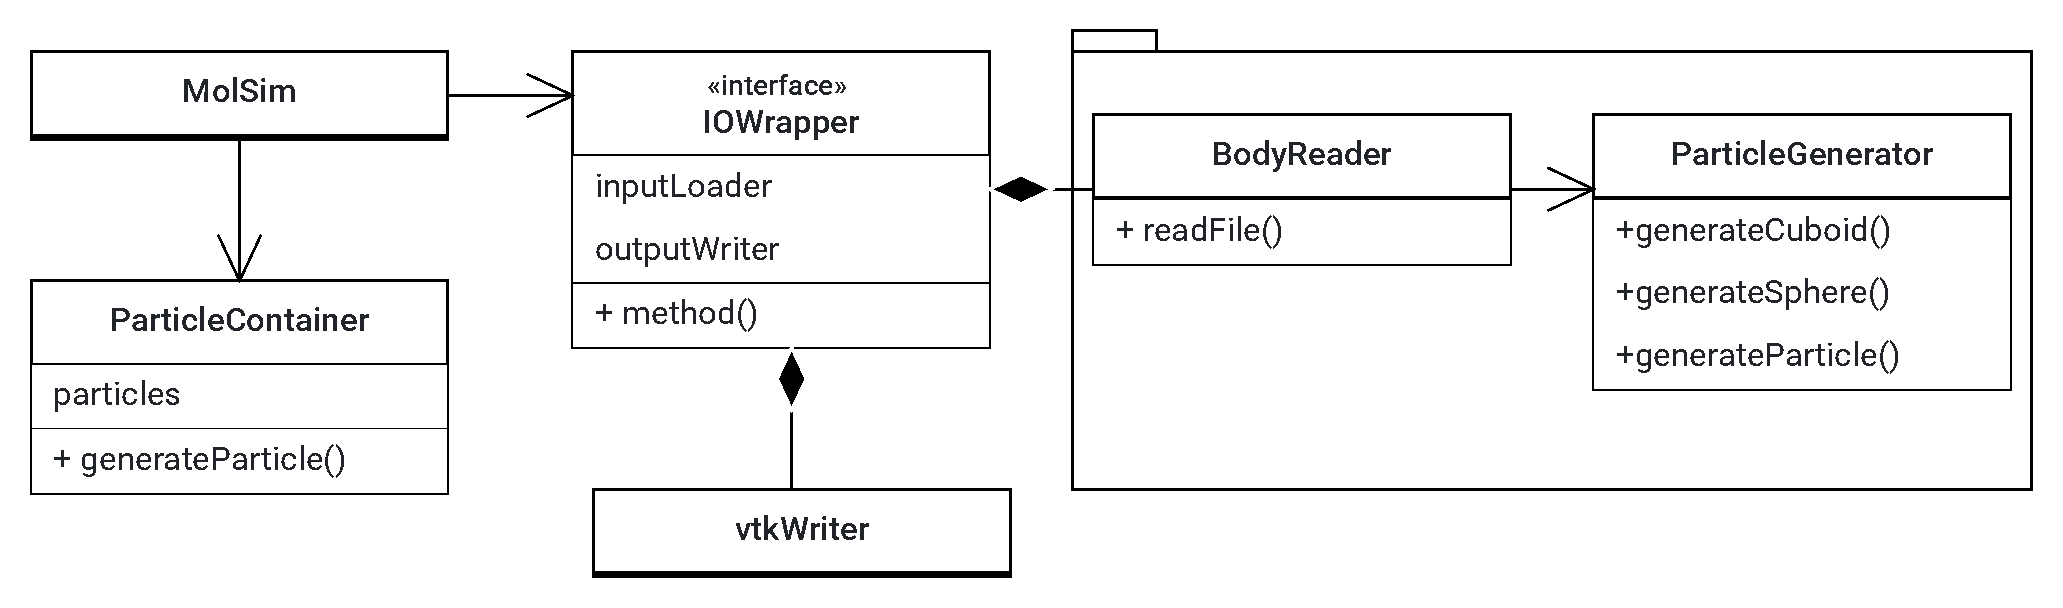
\includegraphics[width=0.7\linewidth]{IOWrapper}
		\label{fig:iowrapper}
	\end{figure}
	\large
	\centering
	input Loader gets chosen at compile time
	%\begin{itemize}
	%\item inputLoader gets chosen at compile time
	%\end{itemize}
\end{frame}


\begin{frame}[fragile]
\frametitle{Input parsing - Definition of Body}
\vspace{0.7cm}

\begin{lstlisting}[language=C++]
enum Shape {cuboid, sphere};

struct Body {
	Shape shape;   
	Eigen::Vector3d fixpoint; 
	Eigen::Vector3d dimensions; 
	double distance;
	double mass;
	Eigen::Vector3d start_velocity;
} ;
\end{lstlisting}
\end{frame}

\begin{frame}
	\frametitle{CI/CD}
	\large
	\begin{itemize}
		\item<1-> Protection of master branch
		\item<2-> Deployment of CI/CD pipeline for \textit{all} branches 
	\end{itemize}
	
\end{frame}


\begin{frame}
	\frametitle{CI/CD}
	\large
	\begin{itemize}
		\item Protection of master branch
		\item Deployment of CI/CD pipeline for \textit{all} branches 
	\end{itemize}
	\Large
	The pipeline consist of:
	\large
	\begin{itemize}
		\item<1-> library installation
		\item<2-> build process
		\item<3-> sanitizers
		\item<4-> unit tests for every major component
	\end{itemize}
\end{frame}

\begin{frame}[fragile]
	\frametitle{CI/CD}
	\begin{lstlisting}
		name: Build and Gtest
		on:
		push:
		branches:
		- '**'        # matches every branch
		pull_request:
		branches: ["master"]
		env:
		#Customize CMake build type here from [Debug;Release;RelWithDebInfo;MinSizeRel]
		BUILD_TYPE: Release	
	\end{lstlisting}
\end{frame}

\begin{frame}[fragile]
	\frametitle{CI/CD}
	
	\begin{lstlisting}
		jobs:
		build_and_gtest:
		runs-on: ubuntu-latest
		steps:
		- uses: actions/checkout@v3
		- name: Install libxerces-c
		run: sudo apt install libxerces-c-dev
		- name: Set up GCC
		run: |
		sudo add-apt-repository -y ppa:ubuntu-toolchain-r/test
		sudo apt install -y gcc-11 g++-11
		- name: Configure CMake
		run: cmake -D CMAKE_C_COMPILER=gcc-11 -D CMAKE_CXX_COMPILER=g++-11 -B ${{github.workspace}}/build -DCMAKE_BUILD_TYPE=${{env.BUILD_TYPE}}
		- name: Build
		working-directory: ${{github.workspace}}/build
	\end{lstlisting}
\end{frame}

\begin{frame}[fragile]
	\frametitle{Logging}
	\large
	format:
	\begin{lstlisting}
		[time][level::context] message
	\end{lstlisting}
	
	\begin{figure}
		\centering
		\includegraphics[width=0.7\linewidth]{logging}
		\label{fig:logging}
	\end{figure}
	
	
	\begin{itemize}
		\item 6 different log-levels available
		\item log-level can be chosen via command line input
	\end{itemize}
\end{frame}

\begin{frame}[fragile]
	\frametitle{Performance optimization}
	\large
	Force calculation is the only part relevant to performance
	\begin{lstlisting}[language=C++]
    void calculateFLennardJones() {
	//set all current forces on all particles to 0
	particleContainer.forAllParticles([](Particle &p) {
		p.setOldF(p.getF());
		p.setF({0., 0., 0.});
	});
	
	particleContainer.forAllPairs([](Particle &p1, Particle &p2){
		calculate force 
		
		p1.add_to_F(force);
		p2.add_to_F(-force);
	});
}

	\end{lstlisting}

\end{frame}

\begin{frame}
	\frametitle{Performance optimization - "Gaussian multithreading"}
	\vspace{1.5cm}
	\begin{columns}
		\begin{column}{0.48\textwidth}
	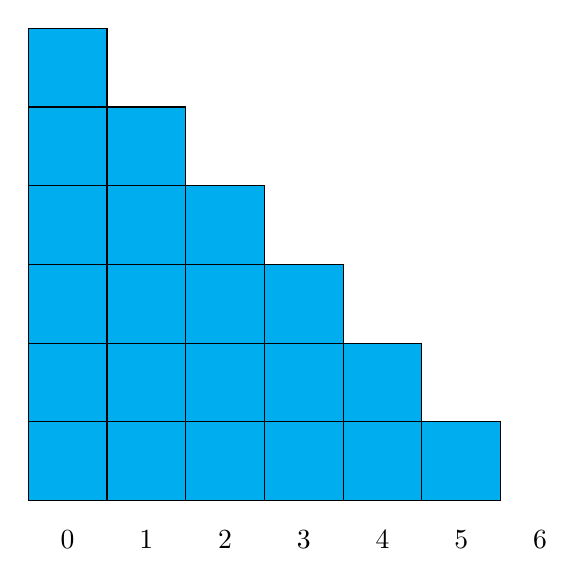
\begin{tikzpicture}
		\foreach \x in {0,...,5}
		\foreach \y in {0,...,\x} 
		\filldraw[draw=black,fill=cyan] (5-\x,\y) rectangle (5-\x+1,\y+1);
		\foreach \k in {0,...,6} {
			\node[] at (\k+0.5, -0.5) {$\k$};
		}	
	\end{tikzpicture}
		\end{column}
		\begin{column}{0.48\textwidth}
	\vspace{-6.5cm}
	\large
	\begin{itemize}
	\item Idea: Force calculation can be multithreaded quite easily 
	\item Evenly distribute Particle-pairs among multiple threads \\
	\item One rectangle represents one necessary force-calculation where $\min(p1,p2)$ is the number displayed below
	\end{itemize}
		\end{column}
	\end{columns}	
\end{frame}

\begin{frame}
	\frametitle{The OpenMP-approach}
	
	\begin{figure}
		\centering
		\includegraphics[width=0.53\linewidth]{alex_code}
		\label{fig:alexcode}
	\end{figure}
	
\end{frame}



\begin{frame}
	\frametitle{Performance optimization - "Gaussian multithreading"}
		\vspace{1.5cm}
		\begin{columns}
		\begin{column}{0.48\textwidth}
			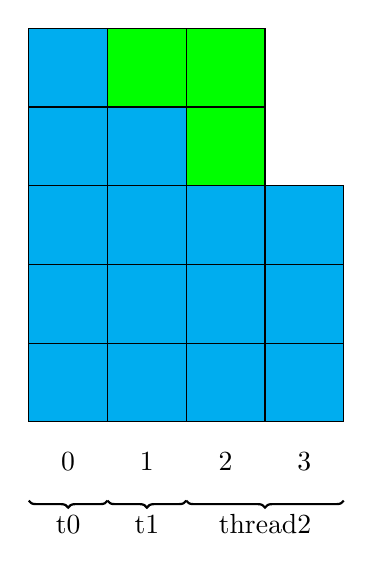
\begin{tikzpicture}
	\foreach \x in {0,...,2}
		\foreach \y in {0,...,2} 
			\filldraw[draw=black,fill=cyan] (\x,\y) rectangle (\x+1, \y+1);
	\foreach \k in {0,...,3} {
		\node[] at (\k+0.5, -0.5) {$\k$};
	}	
	\foreach \x in {0,...,2}
		\foreach \y in {0,...,\x} 
			\filldraw[draw=black,fill=cyan] (2-\x,\y+2) rectangle (2-\x+1, \y+1+2);
	\filldraw[draw=black,fill=green] (1,4) rectangle (2,5);
	\filldraw[draw=black,fill=green] (2,4) rectangle (3,5);
	\filldraw[draw=black,fill=green] (2,3) rectangle (3,4);
	\filldraw[draw=black,fill=cyan] (3,0) rectangle (4,1);
	\filldraw[draw=black,fill=cyan] (3,1) rectangle (4,2);
	\filldraw[draw=black,fill=cyan] (3,2) rectangle (4,3);
	\draw [decorate,decoration = {brace}, thick] (1,-1) -- (0,-1);
	\node[]at (0.5, -1.3){t0};
	\draw [decorate,decoration = {brace}, thick] (2,-1) -- (1,-1);
	\node[]at (1.5, -1.3){t1};
	\draw [decorate,decoration = {brace}, thick] (4,-1) -- (2,-1);
	\node[]at (3.0, -1.3){thread2};
	
	\end{tikzpicture}
		\end{column}
		\begin{column}{0.48\textwidth}
			\vspace{-6.5cm}
			\large
			\begin{itemize}
				\item Create "Gaussian rectangle"' as good as possible and distribute the resulting blocks
				\item Threads use personal accumulators
				\item Accumulators get added in the end
			\end{itemize}
		\vspace{1.5cm}
		\Large
			In the end outsourcing the problem to OpenMP turned out to be much easier
		\end{column}
	\end{columns}
\end{frame}

\begin{frame}
	\frametitle{Performance optimization - Refactoring of ParticleContainer and SIMD}
	\large
	\vspace{1cm}
	\begin{itemize}
	\item<1-> Utilization of seperate vectors for forces, velocities and positions instead of using one struct
	\item<2-> Flattening of the two-dimensional Vectors: \\
	std::vector<Eigen::Vector3d> $\rightarrow$ std::vector<double> \\
	\item<3->[]\Large $\longrightarrow$ Perfect setup for SIMD-Instructions (no working version implemented yet)(with 32 byte alignment)
	
	\end{itemize}
	
\end{frame}

\begin{frame}
	\frametitle{Laptops sometimes do explode, and other lessons we had to learn}
	\large
	\begin{itemize}
	\item<1-> Get yourself familiar with alternative options available to not completely disrupt your workflow
	\item<2-> Create backups!
	\item<3-> People are nice, ask for help
	\item<4->  Get an overview over the already existing functionality and helper functions
	\item<5->  Communicate on interfaces, project structure, etc.
	\item<6-> Documentation and Code examples are your friend
	\end{itemize}
	\item<7-> Don't forget to update your documentation
	
\end{frame}

%\frame[label=blah]{
%	\begin{center}%
%		\href{run:/usr/local/bin/mplayer -fs standard-benchmark.mp4}{
%		\includegraphics[scale=0.25]
%		{Assignment2_Presentation.pdf}}

%		\includemovie{.85\textheight}{.85\textheight}{standard-benchmark.mp4}%
%	\end{center}%
%	\note{%
%		\begin{itemize}
%			\item blah
%			\item blah
%		\end{itemize}
%	}%
%}


%%%%%%%%%%%%%%%%%%%%%%%%%%%%%%%%%%%%%%%%%%%%%%%%%%%%%
%% Folie: Gültigkeit der Masterfolien              %%
%%%%%%%%%%%%%%%%%%%%%%%%%%%%%%%%%%%%%%%%%%%%%%%%%%%%%
